\documentclass[12pt,a4paper]{report}
\usepackage{amsmath,amsthm,amssymb,mathrsfs,graphicx,}
\allowdisplaybreaks


\newtheorem{theorem}{Theorem}
\newtheorem{definition}{Definition}
\newtheorem{example}{Example}
\newtheorem{corollary}{Corollary}
\newtheorem{lemma}{Lemma}
\newtheorem{proposition}{Proposition}
\newtheorem{remark}{Remark}
\newtheorem{algorithm}{Algorithm}

\renewcommand{\baselinestretch}{1.5}


\begin{document}

%%This needs to be put here
One observation is the high density of cones within the fan, especially around "difficult" orderings such as the lex ordering. This causes a significant problem where we have to explicitly calculate cones that are difficult to calculate. On top of this, since the density of the cones are so high, these complex cones are, relative to the Groebner fan as a whole, very small. This leads to the situation where a significant amount time is spent on calculating the fans, but the distance walked for each fan is minimal (distance traversed is less or equal to 0.001 per fan). This causes a significant decrease in performance compared to any straight line walk.
%%

\chapter{Tracking Groebner Walk Progress}
Most of the implementations of the Groebner Walk in various CASes (Computer Algebra Systems) do not have any sort of tracking, e.g. in the form of progress or status bars, of the Groebner Walk. This means that, after initiating computation but before the algorithm terminates, there is no indication of the remaining distance that the Groebner Walk needs to traverse, as well as any estimation of how long the remaining distance will take to traverse. This is especially frustrating given the difficulty and computational complexity of Groebner Bases in general, especially those that encode much more information within them e.g. Bases with lexicographical ordering.

Again, like the Groebner Walk algorithm itself, there does not exist one right way to implement this. However, we would like our tracking progress algorithm to satisfy a few basic functionalities:

%%Make this a little more mathematical?
\begin{enumerate}
    \item Remaining distance measured is  monotonically decreasing.
    \item The algorithm terminates when remaining distance measured is 0.
\end{enumerate}

These are very reasonable assumptions to make. Firstly, to explain the desire to have monotonically decreasing distance, every Groebner Walk algorithm implementation will always try to walk from the starting term order, to the term order we desire. It would not make sense to have the Groebner walk move away from the target term order, so it would also not make sense to see the distance increase during the calculation, as this would imply that it is walking in a nonsensical way. Secondly, having remaining distance equal to zero gives the appearance that the Groebner walk has finished walking to the target term order and has hence terminated. If this was not the case, it would appear that the algorithm had either terminated unexpectedly, or had outputted the wrong Groebner basis.

\section{Barycentric method}
To begin, we could explain a very simple method of measuring distance. It is done in the following fashion:

\begin{enumerate}
    \item Treat each cone $C_{\prec} (I)$ we enter as a single point $c$, that point being the barycentre of the cone.
    \item Distance is measured in a straight line, from the current cones' barycentre $C_{\prec_{1}} (I)$  to the target cones' barycentre $C_{\prec_{2}} (I)$.
\end{enumerate}


The simplest way of measuring this distance would be working in the Euclidean metric.

Hence, we can define the barycentres in coordinate form. Define the current cone barycentre as $c_{cur} = (a_{1}, \cdots, a_{n})$, and the target cone barycentre as $c_{tar} = (b_{1}, \cdots b_{n}$. Then, we can measure the total distance of the line $l$ between $c_{cur}$ and $c_{tar}$ in the following way:
\begin{equation*}
    dist(l) = \sqrt{\sum_{i=1}^{n} (a_{i} - b_{i})^{2}}
\end{equation*}

As we move through into a new cone, the barycentre of the new cone becomes the new $c_{cur}$.

%%%%%%%%%%%%%%%%%%%%%%Good Barycentre
\begin{figure}
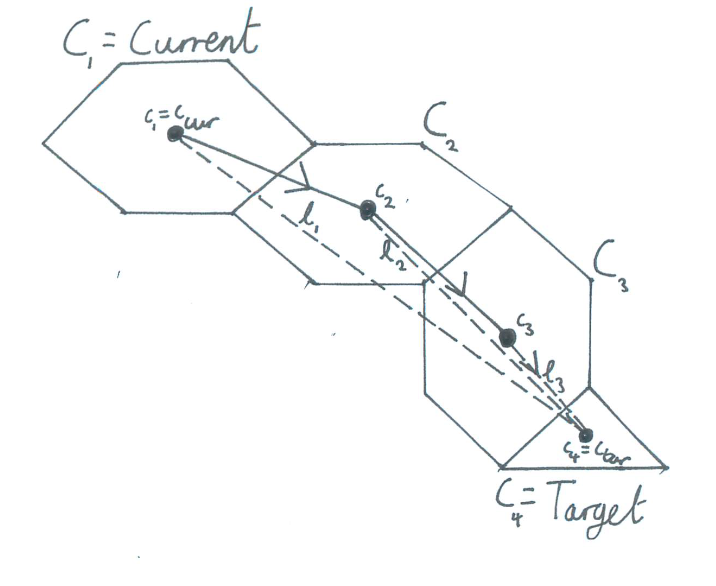
\includegraphics[scale=0.5]{Chapters/images/Barycentre1.png}
\caption{An example of the Barycentric method}
\end{figure}
%%%%%%%%%%%%%%%%%%%%%%%%%%%%%%%%%%%%%%%%

In this example, we start with $C_{1}$ being the current cone, $c_{cur}$ being the current barycentre and $C_{4}$ being the target cone, $c_{tar}$ being the target barycentre. The distance at this step is measured by the distance of dashed line $l_{1}$. Following on, when the walk moves into $C_{2}$, then $c_{2}$ becomes the new $c_{cur}$, and so our distance at this step is dashed line $l_{2}$. We repeat this same process for $C_{3}$ and barycentre $c_{3}$.


This is a very simple way of implementing distance, but it is an important example to show that this simplistic implementation fails to meet either of the basic requirements we had laid out earlier, due to the nature of Groebner cones. The problem here is the representation of a cone reduced to a single point. It is not hard to construct a situation where distance may increase unexpectedly, all we need is a large thin cone and realise that the barycentre would be very far apart from the edges of the adjacent cones, and hence very unrepresentative of the walk as a whole. Another consequence of this is that the algorithm may finish with distance still being a positive, non-zero value.

%%%%%%%%%%%%%%%%%%%%%%Bad Barycentre
\begin{figure}
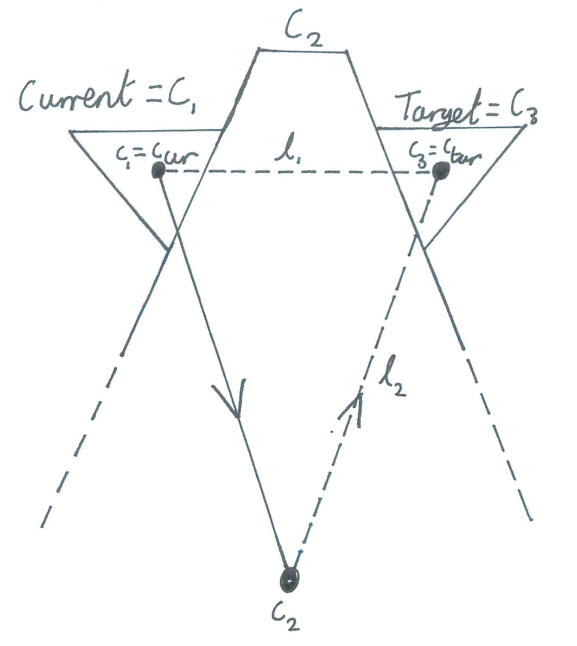
\includegraphics[scale=0.5]{Chapters/images/Barycentre2.png}
\caption{A weakness of the Barycentric method}
\end{figure}
%%%%%%%%%%%%%%%%%%%%%%%%%%%%%%%%%%%%%%%%

Here, in this example, we can see visually that distance of $l_{2}$ is larger of $l_{1}$ despite the fact that cone $C_{2}$ is closer to the target cone than $C_{1}$. This implies that the distance, when walking from cone $C_{1}$, to $C_{2}$ and then $C_{3}$, that instead of having distance decrease monotonically, it instead increases. In this case, the barycentre $c_{2}$ is not representative of the cone as a whole. 

This serves as a good, demonstrative example that tracking progress of the Groebner Walk is a little more difficult to implement as it may first appear, and that our lack of knowledge of the Groebner cone generally makes our lives a little more complicated.

Instead, we will explore a couple other methods of measuring this distance, usually associated with a specific Groebner Walk method.

\section{L1 Ball}
This is the method of measuring distance we used in the facet Orientated method.

We will use projection of L1 ball/unit circle ($|x| + |y| = 1)$, intersected with the positive orthant.

%%Diagram?

%%Is this necessary?
We will determine our straight line to use to calculate distance in the following way. From our starting cone $C_{\prec_{1}} (I)$ we draw a straight line to cone $C_{\prec_{2}} (I)$. When we enter a cone, there are two cases we need to consider. If the face of the new cone $C_{\prec} (I)$ that the line intersects is the closest to $C_{\prec_{2}} (I)$, we continue using this line. However, if there is a closer face we can use that the line does not intersect, we will redraw the straight line to $C_{\prec_{2}} (I)$ from cone $C_{\prec} (I)$ using this new face.

%%Reword this entire section
To calculate this, we do the following:
\begin{itemize}
    \item Given points on a simplex, calculate the norm (absolute sum of points/lead coefficients)
    \item Normalise the vectors by dividing vector by distance.
    \item Distance between two points is: difference between normalised vectors, which is then normed. 
\end{itemize}

We start with two points on a simplex, current and target, which we can denote as $S_{cur} = (a_{1}, \cdots, a_{n})$ and $S_{tar} = (b_{1}, \cdots, b_{n})$. We can then calculate the distance norm by simply calculating $\sum_{i=1}^{n} |a_{i}|$. Then we can normalise this distance onto the unit circle by dividing the vector by the length, calculated by the norm.

Normed vector:
\begin{equation*}
    \frac{\textbf{x}}{\sum_{i=1}^{n} |x_{i}|}
\end{equation*}

Difference between points vector:
\begin{equation*}
   \textbf{x} - \textbf{y} = \frac{\textbf{x}}{\sum_{i=1}^{n} |x_{i}|} - \frac{\textbf{y}}{\sum_{i=1}^{n} |y_{i}|}
\end{equation*}

Hence the distance between these two points is
\begin{equation*}
x - y is \sum_{i=1}^{n} | x_{i} - y_{i} |.    
\end{equation*}

We can create a new vector, which is the difference between these new normalised vectors. We can then calculate the distance by calculating the norm of this new vector.

%%%%%%%%%%%%%%%%%%Norm with two points

\begin{figure}
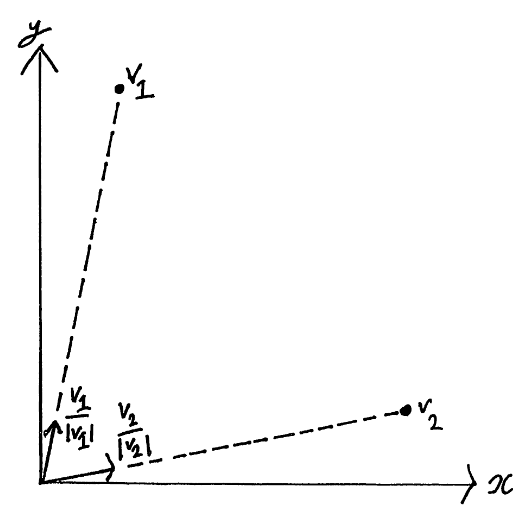
\includegraphics[scale=0.5]{Chapters/images/L1Norm1.png}
\caption{An example of the L1 Norm method}
\end{figure}

%%%%%%%%%%%%%%%%%%%%%%%%%%%%%%%%%%%%%%%%


\section{Straight Line Method}
For this method, we can characterise the current and target point using a hyperbola on the positive orthant.

We can do this in the following way:

\begin{itemize}
    \item Draw a (rectangular) hyperbola, defined by $h = \sum_{x=1}^{n} x_{i} = 1$ in $\mathbb{R^n}$ for variables $x_{1}, \cdots, x_{n}$. For example, in $\mathbb{R^2}$, we have variables $x,y$, so our hyperbola is $xy = 1$.
    \item For a point A, draw a line passing through A and origin O, denoted $l_{1}$.
    \item Find the point of intersection between line $l_{1}$ and the parabola, denote this as $A^{'}$.
    \item Repeat process for point B, to find $B^{'}$.
\end{itemize}

%%Clarify what the hell I mean by "relatively accurate"
Ideally, we would like to measure the distance between $A^{'}$ and $B^{'}$ using the arc length, however there is no closed form expression to calculate this. In this case of $xy = 1$, the arc length is defined by $\int \sqrt{1 + \frac{1}{x^4}} dx$. While this cannot be easily calculated due to lack of a closed form, there are potential ways to estimate this arc length. An example is to calculate $\int 1 + \frac{1}{x^4} dx$ and then square root the result, which is relatively accurate for reasonable $x$ values (i.e. x not too small or large).

Instead of attempting to work with the arc length, we will take the Euclidean distance between points $A^{'}$ and $B^{'}$ instead.

\begin{figure}
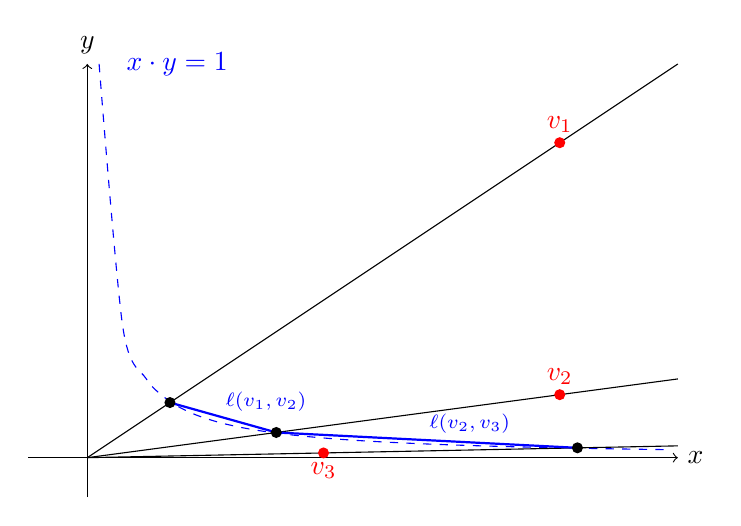
\begin{tikzpicture}[x=1.5cm,y=1cm]
  \draw[->] (-0.5, 0) -- (5, 0) node[right] {$x$};
  \draw[->] (0, -0.5) -- (0, 5) node[above] {$y$};
  \draw[dashed,yscale=0.5, domain=0.1:4.9, smooth, variable=\x, blue] plot ({\x}, {1/\x});
  \node[blue,anchor=west] at (0.25,5) {$x\cdot y=1$};
  \draw[] (0,0) -- (5,5);
  \draw[] (0,0) -- (5,1);
  \draw[] (0,0) -- (5,0.15);
  \coordinate (i1) at (0.7,0.7);
  \coordinate (i2) at (1.6,0.32);
  \coordinate (i3) at (4.15,0.125);
  \coordinate (v1) at (4,4);
  \coordinate (v2) at (4,0.8);
  \coordinate (v3) at (2,0.06);
  \draw[blue,thick] (i1) -- node[anchor=south west,xshift=-1mm,yshift=-0.5mm,font=\scriptsize] {$\ell(v_1,v_2)$} (i2) -- node[anchor=south west,xshift=-1mm,yshift=-0.5mm,font=\scriptsize] {$\ell(v_2,v_3)$} (i3);
  \fill (i1) circle (2pt);
  \fill (i2) circle (2pt);
  \fill (i3) circle (2pt);
  \fill[red] (v1) circle (2pt);
  \fill[red] (v2) circle (2pt);
  \fill[red] (v3) circle (2pt);
  \node[red,above] at (v1) {$v_1$};
  \node[red,above] at (v2) {$v_2$};
  \node[red,below] at (v3) {$v_3$};
  % \draw[scale=0.5, domain=-3:3, smooth, variable=\y, red]  plot ({\y*\y}, {\y});
\end{tikzpicture}
\caption{Example with points v1, v2 and v3}
\end{figure}

In this example, for each point $v_{1}, v_{2}, v_{3}$, they can be represented on the hyperbola and then the distance between these points can be measured using the method we outlined earlier. Note that the distance from $v_{1}$ to $v_{2}$ is, visually, larger than $v_{2}$ to $v_{3}$. However, when measured using the hyperbola, it is clear that the distance of $l(v_{1}, v_{2})$ is smaller than distance of $l(v_{2}, v_{3})$.


\section{Great Circle Distance}
We can also measure distance using circles and geosidics. If we have our start and target point on a circle, we can measure the distance using a geosidic rather than a simple straight line.

However, these geosidic measurements can become unstable and have floating point errors for small distances, since they are based off of the spherical law of cosines. (e.g. $cos(x) \approx 0.999999$ for $x = 0.001$.)

%%Mention something about density of cones?

%%Example of formula

Other formulas that have been conditioned to deal with these small distance floating point errors conversely have problems with antipodal points. Hence we would likely need to implement both formulas, to avoid these errors.

\end{document}